% !TXS template
\documentclass[english]{article}
\usepackage[T1]{fontenc}
\usepackage[utf8]{inputenc}
\usepackage{lmodern}
\usepackage[a4paper]{geometry}
\usepackage{babel}
\usepackage{graphicx}
\usepackage{multicol}
\usepackage{algorithm,algorithmic}
\usepackage{colortbl}

\title{\textbf{MITRO 209 Project Report}}
\author{Quentin Buzet}
\date{January 29, 2023}

\begin{document}

\maketitle
I realized afterwards that we talk about nodes for a tree and vertices for a graph. I'm sorry for this confusion of vocabulary.
\begin{multicols}{2}
\section{Introduction}
\paragraph{}
The aim of this project is to implement in linear time $O(n+m)$ with $n$ the number of nodes and $m$ the number of edges, the 2-approximation algorithm for finding a denset subgraph.
\section{Algorithm}
\paragraph{}
In this section, we are going to see how to implement the 2-approximation algorithm.
\subsection{Reminder}
	\begin{algorithm}[H]
		\caption{2-approximation denset subgraph}
		\begin{algorithmic}
		\STATE $H = G$
		\WHILE{$G$ contains at least one edge} 
			\STATE Let $\nu$ be the node with min degree in $G$
			\STATE Remove $\nu$ and all its edges from $G$
			\IF{$\rho(H) > \rho(G)$}
				\STATE $H \leftarrow G$
			\ENDIF
		\ENDWHILE
		\RETURN H
		\end{algorithmic}
	\end{algorithm}
\subsection{Intuition}
\paragraph{}
To extract the node of minimum degree at each step, we could use a heap but then our implementation will not be in $O(n+m)$ and it could be complicated to maintain the degree of each nodes up to date in our heap when we remove edges.
To achieve a better complexity, we could notice that the degrees can only take values in $[[1,n]]$ and think about another way to sort the degrees.
\paragraph{}
The counting sort is not a comparison sort and could be faster than heap sort for instance, as its complexity is in $O(n+m)$ with $n$ the number of values to sort and $m$ the number of possible values. But it works only if the number of possible value is finite.
\begin{algorithm}[H]
	\caption{Counting sort}
	\begin{algorithmic} 
	\STATE Define the array $count[[0,m]]$
	\FOR{$i=0$ \TO $n-1$}
		\STATE $input =$ the i-th value
		\STATE $count[input] = count[input] + 1$
	\ENDFOR
	\FOR{$i=0$ \TO $i=m$}
		\WHILE{$count[i]\neq0$}
			\PRINT $i$
			\STATE $count[i]=count[i]-1$
		\ENDWHILE
	\ENDFOR
	\end{algorithmic}
\end{algorithm}
\paragraph{}
Thus, we can use the same idea as in the counting sort to extract the node of minimum degree: for each value $\delta$ in $[[1, n]]$ maintain a list of nodes with degree $\delta$ in the current graph.
\paragraph{}
Finally, we have to maitain the table of degrees up-to-date after each deletion.
When we remove a node from the graph, the degree of nodes linked to it will decrease by one and the other nodes will keep the same degree as the previous step.
To remove efficiently a node in its list, we will need a table which store the degree of each nodes in order to know in which list the node is currently and a table which store the position (its pointer) of the node in the list.
\subsection{Data structures}
\paragraph{}
I use C++ to compute the algorithm as it is a fast langage and has a standard librairy.
To process the data I use Python as it is simple.
\begin{itemize}
	\item I store the graph as an adjacency list {\bf adjList}, it take $O(n+m)$. We could not use an adjacency matrix as the complexity will be $O(n^2)$ just for reading the graph.
	\item A table {\bf nodesOfDegree} which stores the lists of nodes with degree $\delta$ with $\delta \in [[0,n]]$. I use lists at it allow us to add or remove a node in $O(1)$.
	\newline I use a {\it vector<list<int>{}>} to do this.
\end{itemize}
\paragraph{}
As explained, before we will need some other informations to find a node and remove it efficiently in nodesOfDegree.
\begin{itemize}
	\item A table {\bf degreeOfNode} which stores the degree of each node.
	\newline I use a {\it vector<int>} to do this.
	\item A table {\bf posOfNode} which stores the position of each node.
	\newline I use a {\it vector<list<int>::iterator>} to do this. An iterator is like a pointer for list in C++. This information is necessary to remove a node in $O(1)$ otherwise it would take $O(n)$.
\end{itemize}
\subsection{Implementation and Complexity}
\paragraph{}
First, I obviously read the data and initialize the graph. It takes $O(n+m)$. 
\paragraph{}
Then, I compute the table nodesOfDegree. To do this, I get for each node its degree by using the adjancy list, (it's just nodesOfDegree[node\_i].size()). It takes $O(\delta(\nu))$ for a single node $\nu$ ; as we do this for all the nodes the total complexity is $O(\sum_{\nu \in G} \delta(\nu)) = O(2m)$. At the same, time I initialize degreeOfNode and posOfNode in $O(n)$ and I find the minimum degree.
\paragraph{}
We can't update the graph at each step of the algorithm as the pseudo-code may suggest because copying the graph takes $O(n+m)$.
That's why, I maintain a table {\bf trace} which stores the order in which I remove the nodes in the graph. Initizalied in $O(n)$. Thanks to this table, I could suppress the nodes at the end of the algorithm and find the 2-approximation of the densest subgraph. The suppressions in the graph are simulate by the well use of nodesOfDegree. \hfill
\paragraph{}
Then I do $n$ iterations:
\begin{itemize}
	\item First, I find the minimum degree (I call it {\bf minDegree}) in the graph. At the next iteration, the minimum degree can decrease by one, as we could have remove an edge linked a node with the same degree. If there is no node with such a degree we increment the degree until we find a node. Checking if a list is empty is $O(1)$. Finding a node of minimum degree at step t could take up to $\delta(\nu_{minDegree(t)}))$ incrementations. Over all the iterations, the total complexity will be $O(\sum_{\nu \in G}{\delta(\nu)}) = O(2m)$.
	\item Then, I take a node of minimum degree (I name it {\bf processNode}) in the graph (the last node in the list nodesOfDegree[minDegree]) in $O(1)$ and I supress it in $O(1)$ thanks to the data structures I defined before
	\item Finally, I update the degrees of nodes linked to the node I remove. For one node, this is performed in $O(1)$ thanks to the data structures I have chosen. \newline
	To do this, first, I remove the node from its degree list, then I decrease its degree by 1 in degreesOfNode and I put it in the new corresponding degree list. Finally I conserve an iterator of its position in posOfNode. \newline There are $\delta(processNode)$ edges to remove. Over all the iterations, the total complexity will be $O(\sum_{\nu \in G}{\delta(\nu)}) = O(2m)$.
\end{itemize}
\paragraph{}
We compute the 2-approximation of the densest subgraph from trace in $O(n+m)$.
$O(n)$ operations to mark the nodes deleted.
$O(n+m)$ operations to traverse the graph and print the remaining edges.
\paragraph{}
Thus, the complexity of our implementation is $O(n+m)$.
\section{Simulation}
\subsection{Pratical considerations}
\paragraph{}
{\it graphs.txt} contains the paths to all the graphs on which the algorithm will perform. For each of them, it is required to precise whether the graph is already given with the reciprocal arc or not. In the first case, the boolean value must be 1, in the second one, 0.
The first line is just the number of graphs in the file.
\paragraph{}
In {\it main.cpp}, there are some printing options at the beging of the file.
Files {\it txt.cpp} and {\it csv.cpp} could be useful to transform a graph to the required format and indexed it correctly. 
\paragraph{}
{\it main.cpp} reads graph in the format:
\newline nbNodes nbEdges
\newline node1 node2
\newline ...
\paragraph{}
To know the datasets I use, check {\it data/datasets.txt}.
\paragraph{}
The algorithm produces an output file {\it results/results.csv} containing the results of the benchmarks.
\subsection{Results}
\paragraph{}
I obtain the following results on 2-approximations:
\newline\newline
\begin{tabular}{|c|c|c|c|}
\hline
\rowcolor{yellow} \bf graph & \bf n & \bf density & \bf time \\
\hline
ca-AstroPh & 1302 & 29.5 & 0.034 \\
\hline
ca-HepPh & 239 & 118.9 & 0.022 \\
\hline
com-amazon & 24990 & 3.83 & 0.41
\\
\hline
com-dblp & 114 & 56.5 & 0.40 \\
\hline
as20000102 & 588 & 4.35 & 0.003 \\
\hline
HR & 6775 & 16.4 & 0.14
\\
\hline
HU & 77 & 8.58 & 0.072 \\
\hline
RO & 426 & 5.02 & 0.041 \\
\hline
large\_twitch &	4207 & 137.32 &	3.23 \\
\hline	
\end{tabular}
\newline
\paragraph{}
Data have been processed using Python and the linear model provided by the librairy scikit-learn.
I import the data with pandas and I visualize them thanks to matplotlib.
\paragraph{}
With all the previous graphs and some others:
\begin{figure}[H]
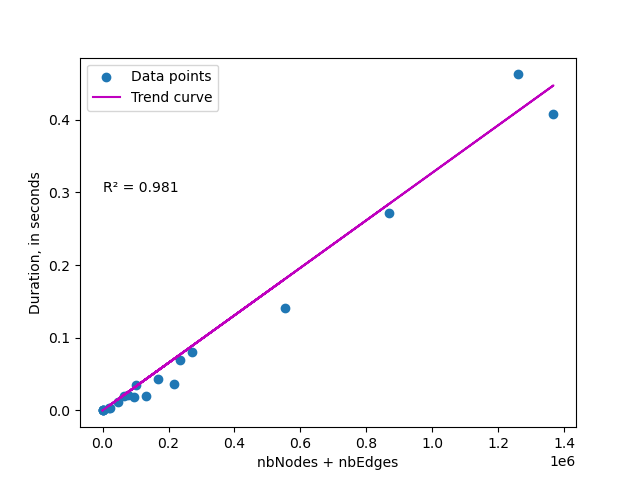
\includegraphics[scale=0.43]{"../results/n+m.png"}
\end{figure}
Without including the large\_twitch\_edges graph to see better this other points, I obtain : 
\begin{figure}[H]
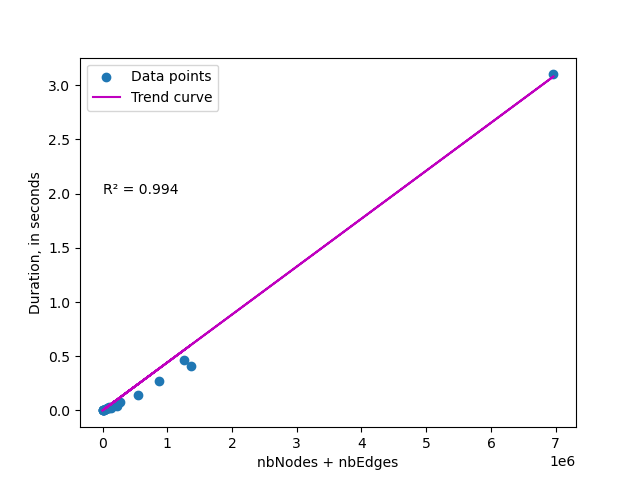
\includegraphics[scale=0.43]{"../results/n+m_large.png"}
\end{figure}
\vfill
The linear model in $n+m$ fit my data as the coefficient of determination is close to 1. I conclude the algorithm implemented here is a O(n+m).
\section{Conclusion}
\paragraph{}
In this paper, I explained how to implement the 2-approximation algorithm for finding denset subgraph and I showed both theorically and experimentally that it runs in $O(n+m)$.
\vfill
\end{multicols}
\end{document}
